%
% File coling2020.tex
%
% Contact: feiliu@cs.ucf.edu & liang.huang.sh@gmail.com
%% Based on the style files for COLING-2018, which were, in turn,
%% Based on the style files for COLING-2016, which were, in turn,
%% Based on the style files for COLING-2014, which were, in turn,
%% Based on the style files for ACL-2014, which were, in turn,
%% Based on the style files for ACL-2013, which were, in turn,
%% Based on the style files for ACL-2012, which were, in turn,
%% based on the style files for ACL-2011, which were, in turn,
%% based on the style files for ACL-2010, which were, in turn,
%% based on the style files for ACL-IJCNLP-2009, which were, in turn,
%% based on the style files for EACL-2009 and IJCNLP-2008...

%% Based on the style files for EACL 2006 by
%%e.agirre@ehu.es or Sergi.Balari@uab.es
%% and that of ACL 08 by Joakim Nivre and Noah Smith

\documentclass[11pt]{article}
\usepackage{coling2020}
\usepackage{times}
\usepackage{url}
\usepackage{latexsym}
\usepackage{graphicx}
\usepackage{array}
\usepackage{booktabs}
\usepackage{multirow}
\usepackage{multicol}
\usepackage{subfig}
% \usepackage{subtable}
% \usepackage{subcaption}

\newcommand{\tabone}{
    \begin{tabular}{lr}
    \toprule
    \textbf{Domain}  & \multicolumn{1}{l}{\textbf{QSs}} \\
    \midrule
    External Relations & 6,580 \\
    Freedom and Democracy & 4,700 \\
    Political System  & 10,557 \\
    Economy & 24,757 \\
    Welfare and Quality of Life & 30,750 \\
    Fabric of Society  & 11,099 \\
    Social Groups  & 9,910 \\
    Not categorized & 1,328 \\
    \bottomrule
    \end{tabular}
}

\newcommand{\tabtwo}{
    \begin{tabular}{lr}
    \toprule
    \textbf{Country} & \multicolumn{1}{l}{\textbf{QSs}} \\
    \midrule
    Australia & 10,370 \\
    Canada & 3,047 \\
    Great Britain & 14,839 \\
    Ireland & 25,352 \\
    New Zealand & 28,561 \\
    South Africa & 6,423 \\
    United States  & 10,819 \\
    \bottomrule
    \end{tabular}
}


%\setlength\titlebox{5cm}
%\colingfinalcopy % Uncomment this line for the final submission

% You can expand the titlebox if you need extra space
% to show all the authors. Please do not make the titlebox
% smaller than 5cm (the original size); we will check this
% in the camera-ready version and ask you to change it back.


\title{Predicting Policy Domains from Party Manifestos with BERT and Convolutional Neural Networks}

\author{Allison Koh \\
  Hertie School of Governance \\
  Friedrichstraße 180 \\
  10117 Berlin, Germany \\
  {\tt koh@hertie-school.org} \\\And
  Daniel Boey \\
  Hertie School of Governance \\
  Friedrichstraße 180 \\
  10117 Berlin, Germany \\
  {\tt danielboeyks@gmail.com} \\\And
  Hannah Bechara \\
  Hertie School of Governance \\
  Friedrichstraße 180 \\
  10117 Berlin, Germany \\
  {\tt bechara@hertie-school.org} \\}

\date{\today}

\begin{document}
\maketitle
\begin{abstract}
  Hand-labeled political texts are often required in empirical studies on party systems, coalition building, agenda setting, and many other areas in political science research. While hand-labeling remains the standard procedure for analyzing political texts, it can be slow and expensive, and subject to human error and disagreement. Recent studies in the field have leveraged supervised machine learning techniques to automate the labeling process of electoral programs, debate motions, and other relevant documents. We build on current approaches to label shorter texts and phrases in party manifestos using a pre-existing coding scheme developed by political scientists for classifying texts by policy domain and policy preference. Using labels and data compiled by the Manifesto Project, we make use of the state-of-the-art Bidirectional Encoder Representations from Transformers (BERT) in conjunction with Convolutional Neural Networks (CNN) and Gated Recurrent Units (GRU) to seek out the best model architecture for policy domain and policy preference classification. We find that our proposed BERT-CNN model outperforms other approaches for the task of classifying statements from English language party manifestos by major policy domain.
  %However, there is room for improvement for employing these techniques for classifying these texts by the more fine-grained policy preference codes.
%   In this paper, we demonstrate the superior performance of incorporating deep language representation models into classifying political texts. In particular, using the state-of-the-art Bidirectional Encoder Representations from Transformers (BERT) in conjunction with convolutional neural networks yields the best predictions for classifying English language statements parsed from party manifestos.
  % Using labels and data compiled by the Comparative Manifesto Project, this paper makes use of the state-of-the-art Bidirectional Encoder Representations from Transformers (BERT) in conjunction with Convolutional Neural Networks and Gated Recurrent Units to seek the best model architecture for policy domain classification.
  % On all English manifestos available ($n_{\mathrm{sentences}}=99,681$), our BERT-CNN model achieved a F1-Micro score of 0.59 for classifying major policy domains.
\end{abstract}

\section{Introduction}
\label{intro}

% The following footnote without marker is needed for the camera-ready
% version of the paper.
% Comment out the instructions (first text) and uncomment the 8 lines
% under "final paper" for your variant of English.
% %
%\blfootnote{
%     %
%     % for review submission
%     %
    % \hspace{-0.65cm}  % space normally used by the marker
    % Place licence statement here for the camera-ready version. See
    % Section~\ref{licence} of the instructions for preparing a
    % manuscript.
%     %
%     % % final paper: en-uk version
%     %
%     % \hspace{-0.65cm}  % space normally used by the marker
%     % This work is licensed under a Creative Commons
%     % Attribution 4.0 International Licence.
%     % Licence details:
%     % \url{http://creativecommons.org/licenses/by/4.0/}.
%     %
%     % % final paper: en-us version
%     %
%     \hspace{-0.65cm}  % space normally used by the marker
%     This work is licensed under a Creative Commons
%     Attribution 4.0 International License.
%     License details:
%     \url{http://creativecommons.org/licenses/by/4.0/}.
%}

During campaigns, political actors communicate their position on a range of key issues to signal campaign promises and gain favor with constituents. %Studies have shown that political parties mostly keep their campaign promises across platforms, time, countries and regimes in North America and Europe ~\cite{petry2009measuring,ringquist2004lies}.
Whilst identifying the political positions of political actors provides no certainty with regards to whether they act upon their policy preferences, it remains essential to understanding their intended political actions. This is why policy preferences---or positions on specific policy issues expressed in speech or text---have been extensively analyzed within the relevant political science literature ~\cite{abercrombie2019policy,budge2001mapping,lowe2011scaling,volkens2013mapping}. Methods employed to investigate the policy preferences of political actors include analysis of roll call voting, position extraction from elite studies or regular surveys, expert surveys and hand-coded analysis and computerized text analysis ~\cite{debus2009estimating}. Studies that utilize political manifestos, electoral speeches, and debate motions often rely on the availability of machine-readable documents that are labeled by policy domain or policy preference.

Quantitative methods, especially in the field of natural language processing, have enabled the development of more scalable methods for predicting policy preferences. These advancements have enabled political scientists to analyze political texts and estimate their positions over time ~\cite{nanni2016topfish,zirn2016classifying}. To better understand the political positions of political actors, many social science researchers have turned to hand-labeling political documents, such as parliamentary debate motions and party manifestos. Much of the previous work on analyzing political texts relies on hand-labeling documents \cite{abercrombie2018sentiment,gilardi2009learning,krause2011policy,simmons2004globalization}. Yet, the analysis of political documents in this field stands to benefit from automating the coding of texts using supervised machine learning. Most recently, neural networks and deep language representation models have been employed in state-of-the-art approaches to automatic labeling of political texts by policy preference.

In this paper, we present a deep learning approach to classifying labeled texts and phrases in party manifestos, using the coding scheme and documents from Manifesto Project ~\cite{volkens2019manifesto}.
%In this paper, we build on labeled texts and phrases in party manifestos using the coding scheme and documents from the Manifesto Project ~\cite{volkens2019manifesto}.
%In particular, we employ neural networks and deep language representation models to classify texts by policy domain and policy preference, based on a coding scheme established by the Manifesto Project ~\cite{volkens2019manifesto}.
We use English-language texts from the Manifesto Project Corpus, which divides party manifestos into statements---or \emph{quasi-sentences}---that do not span more than one grammatical sentence. Based on the state-of-the-art deep learning methods for text classification, we propose using Bidirectional Encoder Representations from Transformers (BERT) combined with neural networks to automate the task of labeling political texts. We compare our models that combine \textsc{Bert} and neural networks against previous experiments with similar architectures to establish that our proposed method outperforms other approaches commonly used in natural language processing research when it comes to choosing the correct policy domain and policy preference. We identify differences in performance across policy domains, paving the way for future work on improving deep learning models for classifying political texts. To the best of our knowledge, we offer the most comprehensive application of deep language representation models incorporated with neural networks for document classification of political manifesto statements.

The rest of this paper is structured as follows. In Section \ref{related_work}, we provide a brief overview of the current state-of-the-art in classification of political texts, focusing mainly on detecting policy domains and preference. Section \ref{data} describes the data, going into detail about the Manifesto Project Corpus. Section \ref{methodology} then introduces our classification approach and provides important details of our models and evaluation approach. In Section \ref{results}, we present our results and address some limitations of our system. Finally, Section \ref{conclusion} concludes our findings and sets up a roadmap for future improvements.

%\footnote{Github repo: https://github.com/allisonkoh/nlp-manifesto-classification}

\section{Related Work}
\label{related_work}
Several studies have concentrated on building scaling models that identify the political position of texts ~\cite{glavavs2017cross,laver2003extracting,nanni2019political,proksch2010position}.
%For the task of classifying political texts, many relevant studies in political science have concentrated on building scaling models for identifying the political position of documents ~\cite{glavavs2017cross,laver2003extracting,nanni2019political,proksch2010position}.
Previously, most of the seminal work in this area has overlooked the task of classifying texts by topic or policy area prior to detecting policy preferences associated with the topic.
Over the past couple of years, several studies have addressed the gap in \textit{opinion-topic identification} by classifying text data from political speeches, manifestos, and other documents by topic before predicting policy preference. %~\cite{glavavs2017cross,zirn2016classifying}
Perhaps most relevant to our research is the paper by \newcite{zirn2016classifying}, in which the authors trained and validated an approach to classifying manifestos from the United States into seven policy domains that involved binary classifiers predicting whether sentences that are adjacent to one another belong to the same topic\footnote{The data used in analysis comprises of statements from six Democratic and Republican election manifestos from the 2004, 2008 and 2012 elections in the United States.}. Their proposed approach of optimizing predictions using a Markov Logic framework yielded an average micro-F1 score of .749. \newcite{glavavs2017cross} introduced a multi-lingual classifier for automatically labeling texts by policy domain. For classification of 20,196 English-language manifestos by policy domain, their CNN models yielded an average micro-F1 score of .59.

%Beyond employing methods for classifying political texts by policy domain, classification schemes for automatically labeling texts by policy preference can be expansive. For instance, the Manifesto Project's classification scheme comprises of 57 categories that represent positive or negative sentiments toward individual policy topics ~\cite{mikhaylov2008coder}. The high number of categories included in in the more fine-grained coding schemes points to the necessity of supervised machine learning and other more computationally intensive methods to take on this text classification task.

More recently, studies have employed neural networks and deep language representation models to address the computationally intensive task of classifying political texts into over thirty categories. To take on this ambitious task, \newcite{bilbao2018automatic} included contextual information about individual quasi-sentences, specifically political party and the previous sentence within a manifesto, into multi-scale convolutional neural networks with word embeddings. Their best performing model for classifying 86,500 quasi-sentences from the Manifesto Project Corpus into the seven major policy domains yielded an F1 score of .6532, and their best performing model for classifying quasi-sentences by policy preference yielded an F1 score of .4273.
\newcite{subramanian2018hierarchical} propose employing a hierarchical sequential deep model that captures information from within manifestos as well as contextual information across manifestos to predict the political position of texts. Their best performing hierarchical modeling approach for classifying 86,603 English language quasi-sentences yielded an F1 score of .50.

 %Bilbao-Jayo and Almeida (2018) use multi-scale CNNs with word embeddings and two types of context data as extra features, like the previous sentence in the manifesto and the political party %~\cite{subramanian2018hierarchical}~\cite{devlin2018bert}

\newcite{abercrombie2019policy} used deep language representation models to detect the policy positions of Members of Parliament in the United Kingdom.
Using motions and manifestos as data sources, the authors employed a variety of methods to predict the policy and domain labels of texts.
They propose utilizing Bidirectional Encoder Representations from Transformers (\textsc{Bert}), with results fine-tuned with party manifestos and the motions themselves. In addition to a final softmax layer, the authors added a CNN model and max-pooling layers to the soft-max layer. they found that the use of \textsc{Bert} demonstrated state-of-the-art performance on both manifestos and motions via supervised pipelines with a Macro-F1 score of 0.69 for their best performing model.
Our work builds on some of the methods proposed in their paper, leveraging neural networks and deep language representation models for classifying political texts.

%Building on recent work that utilizes neural networks and deep language representation models for classifying political texts, this paper introduces an approach for classifying statements from political manifestos into the seven broader policy domains and the fine-grained policy preference classification scheme. In particular, this paper follows some of the methods proposed by Abercrombie et al. \shortcite{abercrombie2019policy}, who worked to detect the policy positions of Members of Parliament in the United Kingdom with deep language representation models. Using motions and manifestos as data sources, they employed a variety of methods to predict the policy and domain labels of texts. They propose utilizing Bidirectional Encoder Representations from Transformers (BERT) with a final soft-max model in one and added a CNN and max-pooling layers in addition to the soft-max layer. %They also fine-tuned the results of the aforementioned BERT Model by first training it on party manifestos and then on the motions.
%Ultimately, they found that the use of BERT demonstrated state-of-the-art performance on both manifestos and motions via supervised pipelines. %,with a Macro-F1 score of 0.69 for their best performing model.
%Overall, their work points to the effectiveness of deep language representation models combined with neural networks in predicting policy preferences from political texts.

\section{The Manifesto Project Corpus}
\label{data}

The Manifesto Project Corpus\footnote{\url{manifesto-project.wzb.eu}} ~\cite{volkens2019manifesto} provides information on policy preferences of political parties from seven different countries based on a coding scheme of seven policy domains, under which 57 policy preference codes are manually coded. The Manifesto Project offers data that divides party manifestos into quasi-sentences, or individual statements which do not span more than one grammatical sentence. Quasi-sentences are then individually assigned to categories pertaining to policy domain and preference. The 57 policy preference codes, one of which is ``not categorized'', refer to the position---positive or negative---of a party regarding a particular policy area. The 57 policy preference codes fall into a macro-level coding scheme comprising of 8 policy domain categories. In political science research, the Manifesto Project Corpus is particularly useful for studying party competition, the responsiveness of political parties to constituent preferences, and estimating the ideological position of political elites. While the official classification of manifestos in this dataset has primarily relied on human coders, the investigation of automatically detecting policy positions of the text data is valuable for scaling up the classification of large volumes of political texts available for analysis.

Our final subset of all English-language manifestos comprises of 99,681 quasi-sentences. Table \ref{tbl:desc} illustrates the distribution of English-language manifestos across countries and policy domains. To ensure that the ratio between policy domains remains consistent across policy domains in running our models, we applied a 70/15/15 split between training, validation, and test sets separately for the 8 major categories and the 58 minor categories.

\begin{table}%
  \centering
  \subfloat[][]{\tabone}%
  \qquad
  \subfloat[][]{\tabtwo}
  \caption{Quasi-sentences (QSs) from English language manifestos by policy domain (a) and country (b)}%
  \label{tbl:desc}%
\end{table}

% \begin{table}[htbp]
%   \centering
%     \begin{tabular}{lr}
%     \midrule
%     \textbf{Domain}  & \multicolumn{1}{l}{\textbf{QSs}} \\
%     \midrule
%     External Relations & 6,580 \\
%     Freedom and Democracy & 4,700 \\
%     Political System  & 10,557 \\
%     Economy & 24,757 \\
%     Welfare and Quality of Life & 30,750 \\
%     Fabric of Society  & 11,099 \\
%     Social Groups  & 9,910 \\
%     Not categorized & 1,328 \\
%     \midrule
%     \end{tabular}%
%   \caption{Quasi-sentences (QSs) from English language manifestos by policy domain}
%   \label{tab:major}%
% \end{table}%

% % Table generated by Excel2LaTeX from sheet 'Sheet1'
% \begin{table}[htbp]
%   \centering
%     \begin{tabular}{lr}
%     \midrule
%     \textbf{Country} & \multicolumn{1}{l}{\textbf{QSs}} \\
%     \midrule
%     Australia & 10,370 \\
%     Canada & 3,047 \\
%     Great Britain & 14,839 \\
%     Ireland & 25,352 \\
%     New Zealand & 28,561 \\
%     South Africa & 6,423 \\
%     United States  & 10,819 \\
%     \midrule
%     \end{tabular}%
%   \caption{Quasi-sentences (QSs) from English language manifestos by country}
%   \label{tab:ctry}%
% \end{table}%


%  \begin{figure*}[th!]
%   \centering
%   \includegraphics[width=\linewidth]{figs/1.desc-major.png}
%   \caption{English language manifestos by policy domain}
%   \label{fig:major}
% \end{figure*}
%
%  \begin{figure*}[th!]
%   \centering
%   \includegraphics[width=\linewidth]{figs/1.desc-country.png}
%   \caption{English language manifestos by country}
%   \label{fig:ctry}
% \end{figure*}
%
%  \begin{figure*}[th!]
%   \centering
%   \includegraphics[width=\linewidth]{figs/1.desc-minor-plasma1.png}
%   \caption{Proportion of QSs from each minor category in each policy domain}
%   \label{fig:minor}
% \end{figure*}

% \begin{table*}[t!]
% \centering
% \begin{tabular}{|l|l|l|c|c|c|c|}
% \hline
%  &
%   &
%   &
%   \multicolumn{2}{c|}{\textbf{Major Categories}} &
%   \multicolumn{2}{c|}{\textbf{Minor Categories}} \\ \hline
% \multicolumn{1}{|c|}{Models} &
%   \multicolumn{1}{c|}{\begin{tabular}[c]{@{}c@{}}Text \\ Representation\end{tabular}} &
%   \multicolumn{1}{c|}{Layers} &
%   Epochs &
%   Training Time &
%   Epochs &
%   Training Time \\ \hline
% \textbf{CNN} &
%   \begin{tabular}[c]{@{}l@{}}GloVe Wikipedia\\ w-emb\end{tabular} &
%   \begin{tabular}[c]{@{}l@{}}2 Convolutional Layers (1 per filter)\\ 2 Max Pooling Layers\\ 1 Dropout Layer\\ 1 Linear Layer\end{tabular} &
%   100 &
%   9m 19s &
%   100 &
%   11m 12s \\ \hline
% \textbf{\begin{tabular}[c]{@{}l@{}}BERT-CNN\end{tabular}} &
%   \begin{tabular}[c]{@{}l@{}}Base BERT\\ (uncased)\end{tabular} &
%   \begin{tabular}[c]{@{}l@{}}2 Convolutional Layers (1 per filter)\\ 2 Max Pooling Layers\\ 1 Dropout Layer\\ 1 Linear Layer\end{tabular} &
%   10 &
%   36m 17s &
%   10 &
%   34m 45s \\ \hline
% \textbf{\begin{tabular}[c]{@{}l@{}}BERT-GRU\end{tabular}} &
%   \begin{tabular}[c]{@{}l@{}}Base BERT\\ (uncased)\end{tabular} &
%   \begin{tabular}[c]{@{}l@{}}1 Bidirectional GRU RNN Layer\\ 1 Dropout Layer\\ 1 Linear Layer\end{tabular} &
%   10 &
%   42m 44s &
%   10 &
%   80m 20s \\ \hline
% \end{tabular}
%   \caption{Model specifications of CNN and BERT (CNN and GRU). The loss function for all models was a Cross Entropy Loss function. For the CNN models, there was one convolutional layer per filter size.}
%   \label{tab:modelspec}
% \end{table*}

% \begin{table*}[]
% \begin{tabular}{|c|c|c|c|c|c|c|c|c|}
% \hline
% \textbf{Policy Cat.} & \multicolumn{4}{c|}{\textbf{Major}} & \multicolumn{4}{c|}{\textbf{Minor}} \\ \hline
% \textbf{Statistics} & \textbf{Test Loss} & \textbf{Test Acc.} & \multicolumn{1}{l|}{\textbf{F1 Micro}} & \multicolumn{1}{l|}{\textbf{F1 Macro}} & \textbf{Test Loss} & \textbf{Test Acc.} & \multicolumn{1}{l|}{\textbf{F1 Micro}} & \multicolumn{1}{l|}{\textbf{F1 Macro}} \\ \hline
% \textbf{MNB} &  & 0.553 & 0.553 & 0.398 &  & 0.385	& 0.385 & 0.154\\ \hline
% \textbf{SVM} &  & 0.578 & 0.578 & 0.460 &  & \textbf{0.463} & \textbf{0.463} & \textbf{0.299} \\ \hline
% \textbf{CNN} & 1.177 & 0.589 & 0.589 & 0.466 & 2.136 & 0.454 & 0.454 & 0.273 \\ \hline
% \textbf{BERT-CNN} & \textbf{1.152} & \textbf{0.594} & \textbf{0.593} & \textbf{0.479} & \textbf{2.098} & 0.448 & 0.446 & 0.260 \\ \hline
% \textbf{BERT-GRU} & 1.166 & 0.591 & 0.591 & 0.473 & 2.216 & 0.432 & 0.432 & 0.239 \\ \hline
% \end{tabular}
% \caption{Baseline, CNN and BERT models run with base specifications as detailed in above Table}
% \label{tab:modelresults}
% \end{table*}

%Describe the dataset(s) you are using (provide references). If it's not already clear, make sure the associated task is clearly described.



\section{Experimental Setup} % May change title based on what else i
\label{methodology}


\subsection{Bidirectional Encoder Representations from Transformers (\textsc{Bert})}

Bidirectional Encoder Representations from Transformers (\textsc{Bert}) have proven successful in prior attempts to classify phrases and short texts \cite{devlin2018bert} .
\textsc{Bert}'s key innovation lies in its ability to apply bidirectional training of transformers to language modelling. This state-of-the-art deep language representation model uses a ``masked language model'', enabling it to overcome restrictions caused by the unidirectional constraint.
%We propose incorporating this deep language representation model to classify quasi-sentences from party manifestos by policy domain and policy preference.

Our experiments use the standard pre-trained \textsc{Bert} transformers as the embedding layer in our model.
%We make use of the \textsc{Bert} BASE uncased tokenizer, with the following parameters:
%\\~\\
%\begin{center}
%$\mathrm{BERT}_{\mathrm{BASE}}$:  (L=12, H=768, A=12, TotalParameters=110M)
%\end{center}
%\\~\\~\\
Since \textsc{Bert} is trained on sequences with a maximum lengths of 512 tokens, %inclusive of the start and end of sentence tokens,
 all quasi-sentences with more than 510 words were trimmed to fit this requirement. Pre-trained embeddings were frozen and not trained for the base models. We test two variants of \textsc{Bert}---one incorporating a bidirectional GRU model, and another incorporating CNNs.
%We demonstrate that, between the two \textsc{Bert} models, the \textsc{Bert}-CNN model demonstrates superior performance against bag-of-words approaches and other models that utilize neural networks.
Model specifications and training times for our neural networks and deep language representation models are shown in Table \ref{tab:modelspec} and Figure \ref{fig:tt}.

%Our proposed method incorporates \textsc{Bert} with neural networks, and test two variants of \textsc{Bert} against several baselines, and we demonstrate its superior performance against bag-of-words approaches and other neural network models, including a variant of \textsc{Bert} that incorporates Gated Recurrent Units ~\cite{cho2014learning}.

% Table generated by Excel2LaTeX from sheet 'model-spec1'
\begin{table}[htbp]
  \centering
    \begin{tabular}{lcp{14.75em}c}
    \toprule
    Models & Text Representation & \multicolumn{1}{l}{Layers} & Epochs \\
    \midrule
    CNN   & GloVe Wikipedia w-emb & 2 Convolutional Layers (1 per filter)\newline{}2 Max Pooling Layers\newline{}1 Dropout Layer\newline{}1 Linear Layer & 100 \\
    \midrule
    \textsc{Bert}-CNN & Base \textsc{Bert} (uncased) & 2 Convolutional Layers (1 per filter)\newline{}2 Max Pooling Layers\newline{}1 Dropout Layer\newline{}1 Linear Layer & 10 \\
    \midrule
    \textsc{Bert}-GRU & Base \textsc{Bert} (uncased) & 1 Bidirectional GRU RNN Layer\newline{}1 Dropout Layer\newline{}1 Linear Layer & 10 \\
    \bottomrule
    \end{tabular} \\~\\%
    \caption{Model specifications of neural networks and deep language representation models}
  \label{tab:modelspec}%
\end{table}%

\begin{figure}[h!]
 \centering
 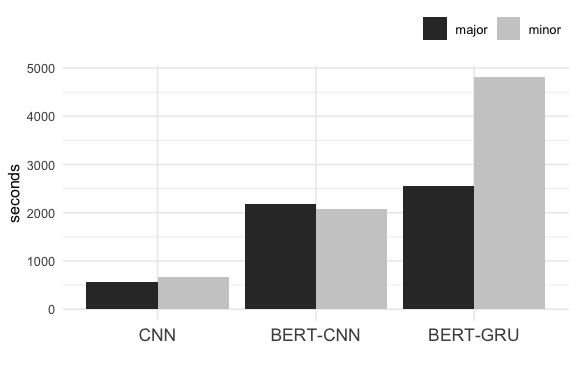
\includegraphics[width=.45\linewidth]{figs/tt.png}
   \caption{Training time for neural networks and deep language representation models for classifying political texts by \textit{major} and \textit{minor} policy domain}
 \label{fig:tt}
\end{figure}

\subsection{\textsc{Bert} with Gated Recurrent Units (GRU)}
First proposed by Cho et al. \shortcite{cho2014learning}, Gated Recurrent Units---formerly referred to as the RNN Encoder-Decoder model---use update gates and reset gates to solve the vanishing gradient problems often encountered in applications of recurrent neural networks ~\cite{kanai2017preventing}. The update gate helps the model determine the extent to which past information is carried on in the model whilst the reset gate determines the information to be removed from the model ~\cite{chung2014empirical}. Hence, it solves the aforementioned problem by not completely removing the new input, instead keeping relevant information to pass on to further subsequent computed states. In our analysis, we employ a multi-layer, bidirectional GRU model from PyTorch\footnote{\url{https://pytorch.org/}}. As shown in Table \ref{tab:modelspec}. The results are subject to a dropout layer prior to classification via a linear layer.


\subsection{\textsc{Bert} with Convolutional Neural Networks (CNN)}


We incorporate CNNs with \textsc{Bert} using the same CNN architecture as our baselines (Table \ref{tab:modelspec}).
The  model utilizes the aforementioned \textsc{Bert} base, uncased tokenizer with convolutional filters of sizes 2 and 3 applied with a ReLu activation function. We use a 1D-max pooling layer, a dropout layer ($N = 0.5$) to prevent overfitting, and a Cross Entropy Loss function.
%A 1D-max pooling function is employed before the output vectors are concatenated. A dropout layer ($N = 0.5$) prevents overfitting. Finally, a linear layer classifies model output into the prediction categories. A Cross Entropy Loss function, preferred for multi-class classification, is utilized to calculate the loss.
%This loss function first takes in the raw, unnormalized scores for each class and employs a softmax function followed by a negative log likelihood loss calculation to calculate the loss.
We employ the model to classify policy domains ($N = 8$) and policy preferences ($N = 58$), each of which includes a category for quasi-sentences that do not fall into this classification scheme. Hereafter, we refer to these classifications as `major' and `minor' categories, respectively. A graphical representation of our model is shown in Figure \ref{fig:BERTCNNfig}.

\begin{figure}[h!]
 \centering
 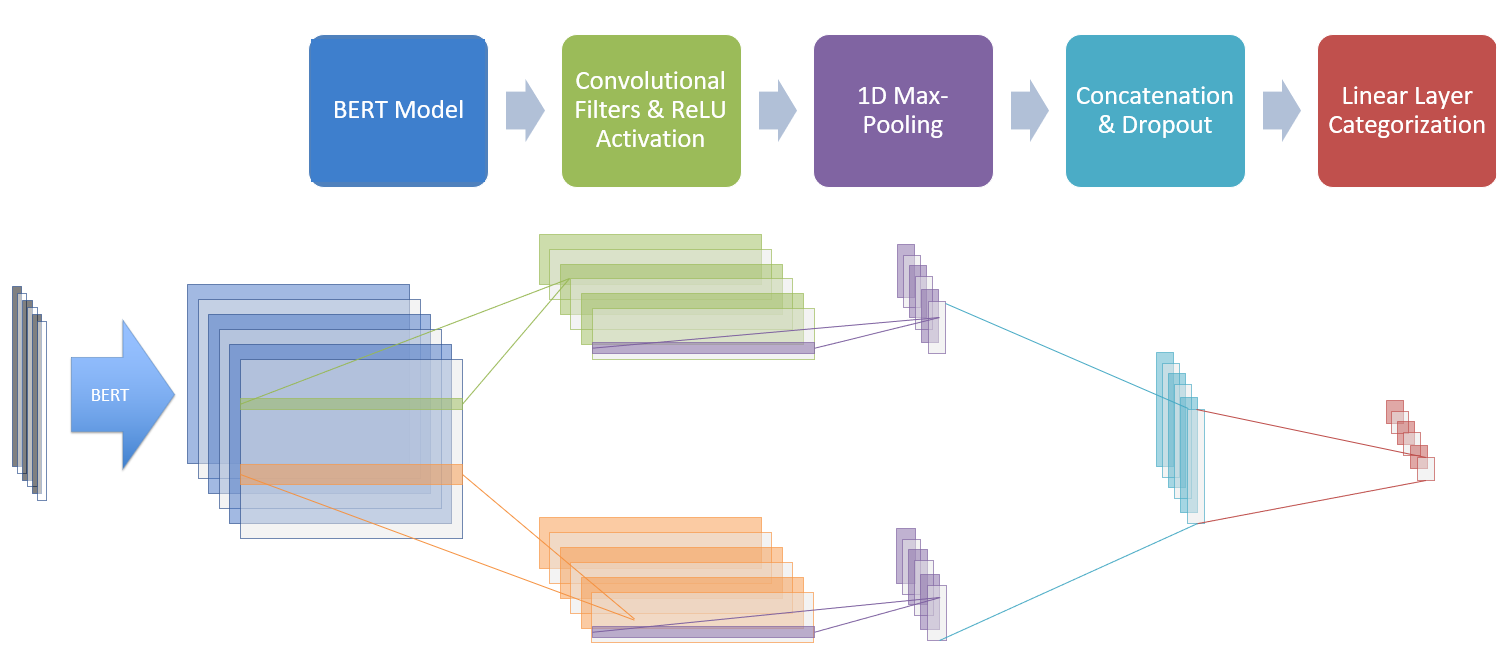
\includegraphics[width=.9\linewidth]{figs/BERTfig3.png}
 \caption{Graphical representation of the base BERT-CNN model to predict major policy domains.}
 \label{fig:BERTCNNfig}
\end{figure}


\subsection{Evaluation}
%In addition to comparing our results against those achieved by \citet{abercrombie2019policy},
We evaluate the performance of our proposed method against several baselines%\footnote{More details on the methods underlying our baseline metrics can be found in the appendix.}
, which include:

\begin{itemize}
    \item \textbf{Multinomial Naive Bayes}: This algorithm, commonly used in text classification, operates on the \emph{Bag of Words assumption} and the assumption of \emph{Conditional independence}.
    \item \textbf{Support Vector Machines} ~\cite{tong2001support}: We used this traditional binary classifier to calculate baselines with the \texttt{SVC} package from \texttt{scikit-learn}\footnote{\url{https://scikit-learn.org/stable/}}, employing a ``one-against-one'' approach for multi-class classification.
    \item \textbf{Convolutional Neural Networks (CNN)} ~\cite{DBLP:journals/corr/Kim14f,lecun1998gradient}: To run this deep learning model, originally designed for image classification, we first made use of pre-trained word vectors trained by GloVe, an unsupervised learning algorithm for obtaining vector representations for words ~\cite{Pennington_Socher_Manning_2014}.%\footnote{See Table \ref{tab:glove} in the appendix for detailed information on pre-trained word embeddings.}.
    % \item \textbf{BERT with Gated Recurrent Units (GRU)} ~\cite{cho2014learning}: The GRU uses update gates and reset gates to adjust the flows of information that determine model output ~\cite{chung2014empirical}. We employ a multi-layer, bidirectional GRU model from \texttt{PyTorch} and subject the results to a dropout layer prior to classification via a linear layer.
\end{itemize}

% \subsection*{BERT with Gated Recurrent Units}
% First proposed by \citet{cho2014learning}, Gated Recurrent Units (originally termed RNN Encoder-Decoder model) uses update gates and reset gates to solve the vanishing gradient problem. The update gate helps the model to determine the extent to which past information is carried on in the model whilst the reset gate determines and forgets the information to be removed from the model \citet{chung2014empirical}. Hence, it solves the aforementioned problem by not completely removing the new input, instead keeping relevant information to passes it on to further subsequent computed states.

% In this model, a multi-layer, bidirectional GRU model from PyTorch was employed. The results were then subject to a dropout layer and then a linear layer for classification (Table \ref{tab:modelspec}).

To evaluate model fit, we utilized \emph{accuracy} and \emph{loss} as key metrics to compare performance of our \textit{CNN} and \textsc{Bert-GRU} baseline and our proposed models (\textsc{Bert+CNN}, \textsc{Bert+GRU}). We calculated the \emph{F1-score} for each model that we ran. In our results, we present both the Macro-F1 score and Micro-F1 score\footnote{The micro score calculates metrics globally whilst the macro score calculates metrics for each label and reports the unweighted mean.}.

% Table generated by Excel2LaTeX from sheet 'base-spec'
\begin{table}[htbp]
  \centering
%   \caption{Add caption}
    \begin{tabular}{llcccc}
    \toprule
    Category & Model & Test Loss  & Test Acc. & Micro-F1 & Macro-F1 \\
    \midrule
    \multirow{5}[2]{*}{Major} & MNB   &   ---  & 0.553 & 0.553 & 0.398 \\
          & SVM   &   ---  & 0.578 & 0.578 & 0.460 \\
          & CNN   & 1.177 & 0.589 & 0.589 & 0.466 \\
          & BERT-GRU & 1.166 & 0.594 & 0.593 & 0.479 \\
          & BERT-CNN & \textbf{1.152} & \textbf{0.591} & \textbf{0.591} & \textbf{0.473} \\
    \midrule
    \multirow{5}[1]{*}{Minor} & MNB   &   ---  & 0.385 & 0.385 & 0.154 \\
          & SVM   &   ---  & \textbf{0.463} & \textbf{0.463} & \textbf{0.299} \\
          & CNN   & 2.136 & 0.454 & 0.454 & 0.273 \\
          & BERT-GRU & 2.216 & 0.432 & 0.432 & 0.239 \\
          & BERT-CNN & \textbf{2.098} & 0.448 & 0.448 & 0.260 \\
    \bottomrule
    \end{tabular} \\~\\
    \caption{Baseline, CNN and \textsc{Bert} models run with base model specifications as detailed in Table \ref{tab:modelspec}}
  \label{tab:modelresults}%
\end{table}%

\subsection{Architecture fine tuning}
%As shown in Table \ref{tab:modelspec} and Figure \ref{fig:tt}, the neural network models we run vary with regards to number of epochs, text representations, layers and training time. The number of epochs were chosen based on the relative time taken to run the models.
%As such, the number of epochs are not regular, especially for the the more computationally intensive \textsc{Bert} models.
We tested different modifications of the CNN and \textsc{Bert} models. For the CNN models, we compared the following modifications:
\begin{itemize}
    \item \textbf{Stemming and Lemmatization}: We test whether stemming or lemmatizing text in the pre-processing steps improves predictions using quasi-sentences from the Manifesto Project Corpus.
    \item \textbf{Dropout rates}: We decreased the dropout rate from 0.5 to 0.25 to determine whether fine-tuning dropout rates yield differences in performance. This is because we initially found that our models were overfitting.
    \item \textbf{Additional linear layer}: An additional linear layer was added prior to the final categorzation linear layer to establish whether ``deeper'' neural networks generate improved predictions.
    \item \textbf{Removal of uncategorized quasi-sentences}: The results from our base models yield lower Macro-F1 scores due to the difficulty of correctly categorizing quasi-sentences that do not fall into any of the 7 policy domains or 57 policy preference codes. We are thus interested in whether predictions improve if the uncategorized quasi-sentences are taken out of the data used for analysis.
\end{itemize}
For the \textsc{Bert} models, we compared the following modifications:
\begin{itemize}
    \item \textbf{Training Embeddings}: For our base \textsc{Bert} models, all training of embeddings were frozen. Therefore, we enable training of the embeddings in this modification to establish how training embeddings contributes to the performance of deep language representation models with this classification task.
    \item \textbf{Training models based on recurrent runs}: We trialed training the \textsc{Bert} models sequentially with different learning rates (LR = 0.001, 0.0005 and 0.0001) of 10 epochs each for a total of 30 epochs in aims to improve the performance of our neural networks and deep language representation models.
    \item \textbf{Large, cased tokenizer}: The \textsc{Bert} Large cased tokenizer was used instead of the \textsc{Bert} BASE uncased tokenizer employed in our base models.

\end{itemize}

\section{Results}
\label{results}


%In addition to comparing our results against those achieved by \citet{abercrombie2019policy},
%We evaluate the performance of our proposed method against several baselines\footnote{More details on the methods underlying our baseline metrics can be found in the appendix.}, which include:

% \begin{itemize}
%     \item \textbf{Multinomial Naive Bayes}: This algorithm commonly used in text classification operates on the \emph{Bag of Words assumption} (position does not matter) and the assumption of \emph{Conditional independence} (feature probabilities are independent given the class).
%     \item \textbf{Support Vector Machines} ~\cite{tong2001support}: We used this traditionally binary classifier to calculate baselines with the \texttt{SVC} package from \texttt{scikit-learn}, employing a ``one-against-one'' approach for multi-class classification.
%     \item \textbf{Convolutional Neural Networks (CNN)} ~\cite{DBLP:journals/corr/Kim14f,lecun1998gradient}: To run this deep learning model, originally designed for image classification, we first made use of pre-trained word vectors trained by GloVe, an unsupervised learning algorithm for obtaining vector representations for words ~\cite{Pennington_Socher_Manning_2014}.%\footnote{See Table \ref{tab:glove} in the appendix for detailed information on pre-trained word embeddings.}.
%     % \item \textbf{BERT with Gated Recurrent Units (GRU)} ~\cite{cho2014learning}: The GRU uses update gates and reset gates to adjust the flows of information that determine model output ~\cite{chung2014empirical}. We employ a multi-layer, bidirectional GRU model from \texttt{PyTorch} and subject the results to a dropout layer prior to classification via a linear layer.
% \end{itemize}

% \subsection*{BERT with Gated Recurrent Units}
% First proposed by \citet{cho2014learning}, Gated Recurrent Units (originally termed RNN Encoder-Decoder model) uses update gates and reset gates to solve the vanishing gradient problem. The update gate helps the model to determine the extent to which past information is carried on in the model whilst the reset gate determines and forgets the information to be removed from the model \citet{chung2014empirical}. Hence, it solves the aforementioned problem by not completely removing the new input, instead keeping relevant information to passes it on to further subsequent computed states.

% In this model, a multi-layer, bidirectional GRU model from PyTorch was employed. The results were then subject to a dropout layer and then a linear layer for classification (Table \ref{tab:modelspec}).

%To evaluate model fit, we utilized \emph{accuracy} and \emph{loss} as key metrics to compare performance of our \textit{CNN} and \textsc{Bert-GRU} baseline and the models from our proposed method of utilizing deep language representation models (\textsc{Bert+CNN}, \textsc{Bert+GRU}). For all models, a Cross Entropy Loss function---often used in multi-class classification---was employed to calculate loss. Average loss per epoch is shown in Table \ref{tab:modelresults}. To evaluate model performance, we calculated the \emph{F1-score} for each model that we ran. In our results, we present both the Macro-F1 score and Micro-F1 score\footnote{The micro score calculates metrics globally whilst the macro score calculates metrics for each label and reports the unweighted mean.}.

As shown in Table \ref{tab:modelresults}, the \textsc{Bert}-CNN model performed best for predicting both major and minor categories compared to the BERT-GRU model and CNN baseline. However, our SVM baseline outperformed the neural network models for predicting minor categories. We believe that the shortcomings of our neural networks and deep language representation models for this text classification task are due to limitations in specifying the number of epochs in training. We also observed overfitting in our models. For instance, with our CNN model, validation loss increased with each additional epoch after a certain number of epochs.
As shown in Figure \ref{fig:minornooverfitting}, training accuracy of this model also increased at the cost of validation accuracy.
However, this was not the case for deep language representation models classifying texts by minor categories. Overall, our results demonstrate that, between the two \textsc{Bert} models, the \textsc{Bert}-CNN model demonstrates superior performance against bag-of-words approaches and other models that utilize neural networks.

\subsubsection*{CNN and \textsc{Bert} Modifications}
Comparing modifications to our CNN models, our results suggest that the base model outperforms most alternative model specifications. As outlined in Table \ref{tab:CNNchange}, reducing the dropout rate to 0.25 improved the model on some indicators marginally. As expected, the removal of uncategorized quasi-sentences yielded improvements in predictions, with a significantly higher Macro-F1 score compared to other model specifications. Based on these results, future work should focus on how model predictions of uncategorized quasi-sentences can be improved, given their random nature.

% Table generated by Excel2LaTeX from sheet 'base-spec'
\begin{table}[htbp]
  \centering
%   \caption{Add caption}
    \begin{tabular}{llcccc}
    \toprule
    Category & Model & Test Loss  & Test Acc. & Micro-F1 & Macro-F1 \\
    \midrule
    \multirow{5}[2]{*}{Major} & MNB   &   ---  & 0.553 & 0.553 & 0.398 \\
          & SVM   &   ---  & 0.578 & 0.578 & 0.460 \\
          & CNN   & 1.177 & 0.589 & 0.589 & 0.466 \\
          & BERT-GRU & 1.166 & 0.594 & 0.593 & 0.479 \\
          & BERT-CNN & \textbf{1.152} & \textbf{0.591} & \textbf{0.591} & \textbf{0.473} \\
    \midrule
    \multirow{5}[1]{*}{Minor} & MNB   &   ---  & 0.385 & 0.385 & 0.154 \\
          & SVM   &   ---  & \textbf{0.463} & \textbf{0.463} & \textbf{0.299} \\
          & CNN   & 2.136 & 0.454 & 0.454 & 0.273 \\
          & BERT-GRU & 2.216 & 0.432 & 0.432 & 0.239 \\
          & BERT-CNN & \textbf{2.098} & 0.448 & 0.448 & 0.260 \\
    \bottomrule
    \end{tabular} \\~\\
    \caption{Baseline, CNN and \textsc{Bert} models run with base model specifications as detailed in Table \ref{tab:modelspec}}
  \label{tab:modelresults}%
\end{table}%


% Table generated by Excel2LaTeX from sheet 'cnn-change'
\begin{table}[htbp]
  \centering
    \begin{tabular}{llccccc}
    \toprule
    Model & Change & Test Loss & Test Acc. & Micro-F1 & Macro-F1 & Epochs \\
    \midrule
    \multirow{6}[1]{*}{CNN} & Base model & 1.177 & \textbf{0.589} & \textbf{0.589} & 0.466 & 100 \\
          & Lemmatized text & \textbf{1.174} & 0.585 & 0.585 & 0.460 & 100 \\
          & Stemmed text & 1.213 & 0.577 & 0.576 & 0.448 & 100 \\
          & Dropout = 0.25 & 1.177 & \textbf{0.589} & 0.588 & \textbf{0.467} & 100 \\
          & Additional layer & 1.180  & 0.586 & 0.586 & 0.462 & 100 \\
          & Removing uncategorized QSs & \textbf{1.136} & \textbf{0.596} & \textbf{0.595} & \textbf{0.535} & 100 \\
    \bottomrule
    \end{tabular} \\~\\
  \caption{Comparing results of modifications to CNN base models for predicting major policy domains}
  \label{tab:CNNchange}%
\end{table}%

%\subsubsection*{\textsc{Bert} Modifications}
While we observed some improvements with modifications to the CNN model, we find that our base \textsc{Bert} models performed best compared to other fine-tuned modifications to model architecture. The results of our base \textsc{Bert} model and alternative model specifications are shown in Table \ref{tab:BERTchange}. Even though it is possible that our base \textsc{Bert} model is best for this classification model, our results could also indicate the presence of over-fitting or the lack of sufficient training available given the low number of epochs.

% Table generated by Excel2LaTeX from sheet 'bert-change'
\begin{table}[htbp]
  \centering
    \begin{tabular}{clccccc}
    \toprule
    \multicolumn{1}{l}{Model} & Change & Test Loss & Test Acc. & Micro-F1 & Macro-F1 & Epochs \\
    \midrule
    \multirow{4}[2]{*}{BERT-GRU} & Base model & \textbf{1.152} & \textbf{0.594} & \textbf{0.593} & \textbf{0.479} & 10 \\
          & Training emb & 1.163 & 0.592 & 0.592 & \textbf{0.479} & 10 \\
          & Recurrent runs, training  & 1.234 & 0.582 & 0.581 & 0.459 & 30 \\
          & Large, uncased & 1.172 & 0.592 & 0.591 & 0.469 & 10 \\
    \midrule
    \multirow{4}[1]{*}{BERT-CNN} & Base model & 1.166 & \textbf{0.591} & \textbf{0.591} & \textbf{0.473} & 10 \\
          & Training emb & 1.167 & 0.587 & 0.587 & 0.458 & 10 \\
          & Recurrent runs, training  & \textbf{1.157} & 0.589 & 0.589 & 0.468 & 30 \\
          & Large, uncased & 1.192 & 0.580 & 0.580 & 0.450 & 10 \\
    \bottomrule
    \end{tabular} \\~\\%
    \caption{Comparing results of modifications to \textsc{Bert} base models for predicting major policy domains}
  \label{tab:BERTchange}%
\end{table}%


\section{Limitations and Analysis}
\label{discussion}

As shown in Figure \ref{fig:majoroverfitting}, we observed overfitting with our major policy domain classification models. Despite employing changes and modifications to our models, including varied dropout rates, architecture fine-tuning and different learning rates, we did not find any variants of the models employed in analysis that would yield significant improvements in performance. We posit that potential improvements on these issues could be resolved by employing transfer learning and appending our sample of English-language manifestos with other political documents, such as debate transcripts.

In contrast, as shown in Figure \ref{fig:minornooverfitting}, we observed little over-fitting in our minor policy domain classification models. Our classifier could benefit from employing transfer learning and appending our sample of manifesto quasi-sentences with other political texts, especially for policy domains with relatively fewer quasi-sentences to train on. It is also important to note that, compared to the more computationally intensive neural networks and deep language representation models, our Multinomial Bayes and SVM baselines did not perform significantly worse. In fact, for the minor categories, the SVM yielded superior performance in some metrics compared to that of the neural network models. Notwithstanding the lack of training of certain models, this may suggest that increasing the model complexity and consequently the computational power required may not necessarily lead to increased model performance.

\begin{figure*}[th!]
  \centering
  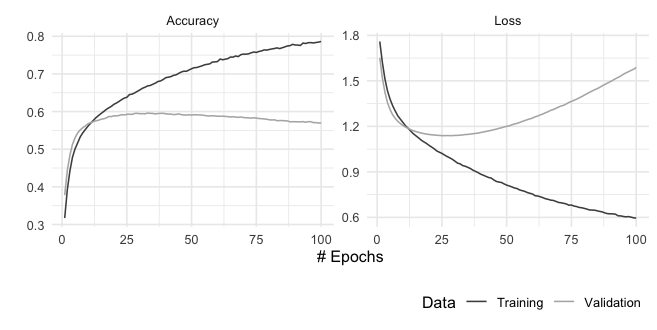
\includegraphics[width=.7\linewidth]{figs/CNNMajor_acc_loss.png}
  \caption{An illustration of overfitting in our CNN model for classifying manifesto quasi-sentences by major policy domain}
  \label{fig:majoroverfitting}
\end{figure*}

\begin{figure*}[h!]
  \centering
  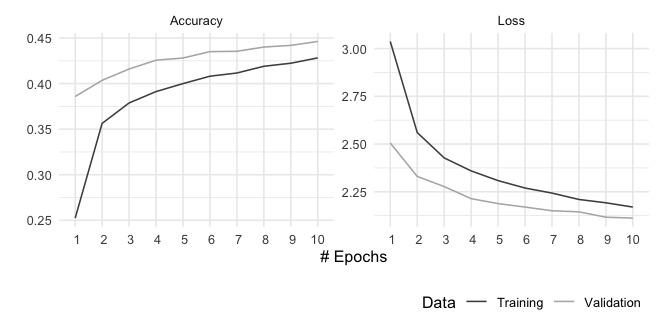
\includegraphics[width=.7\linewidth]{figs/BERTCNNMinor_acc_loss.png}
  \caption{Training and validation metrics for the BERT-CNN model on English language manifestos on minor policy domains}
  \label{fig:minornooverfitting}
\end{figure*}
%

\begin{figure*}[h!]
  \centering
  \includegraphics[width=.8\linewidth]{figs/prf1-major-bw.png}
  \caption{Average precision, recall, and Macro-F1 scores by major category across all models}
  \label{fig:prf1major}
\end{figure*}

Substantially lower Macro-F1 scores across all models point to mixed performance in classification by category. As shown in Figure \ref{fig:prf1major}, we observe high variation in the performance of our classifiers between categories. However,, we observe poor performance in classifying quasi-sentences that do not belong to one of the seven policy domains. For our BERT-CNN model, the easiest categories to predict were ``welfare and quality of life'', ``economy'', and ``freedom and democracy''. The superior performance of predicting the first two categories is not particularly surprising, as a substantial number of quasi-sentences in our sample of English-language party manifestos are attributed to these topics. As shown in Table \ref{tbl:desc}, 30,750 quasi-sentences are attributed to the ``welfare and quality of life'' category and 24,757 quasi-sentences are attributed to the ``economy'' domain.


In contrast, the relatively superior performance of predicting the ``freedom and democracy'' category is surprising. Out of our total sample of $n_{\mathrm{sentences}}=99,681$, only 4,700 documents are attributed to the ``freedom and democracy'' category. Intuitively, the performance of our classifier with this underrepresented policy domain could be attributed to a variety of possible explanations. One possible explanation is the presence of distinct features such as topic-unique vocabulary that do not exist in other categories. Future work on classification of political documents that fall under this category would benefit from looking into features that might distinguish this policy domain from others.

\section{Conclusion}
\label{conclusion}

In this paper, we trained two variants of the state-of-the-art Bidirectional Encoder Representations from Transformers (\textsc{Bert})---one incorporating a bidirectional GRU model, and another incorporating CNNs. We demonstrate the superior performance of deep language representation models combined with neural networks to classify political domains and preferences in the Manifesto Project. Our proposed method of incorporating \textsc{Bert} with neural networks for classifying English language manifestos addresses issues of reproducibility and scalability in labeling large volumes of political texts. As far as we know, this is the most comprehensive application of deep language representation models and neural networks for classifying statements from political manifestos.

We find that using \textsc{Bert} in conjunction with convolutional neural networks yields the best predictions for classifying English language statements parsed from party manifestos. However, our proposed \textsc{Bert}-CNN model requires further fine-tuning to be effective in providing  acceptable predictions to improve on less computationally intensive methods and replace human annotations of fine-grained policy positions. As expected, our proposed approach and baselines perform better for classifying major policy domains over minor categories. We also observe differences in performance between categories. Among the major policy domains, the categories that performed best include ``welfare and quality of life'', ``economy'', and ``freedom and democracy''. The superior performance of the latter category is surprising because it makes up the smallest proportion of quasi-sentences in the Manifesto Project Corpus.
%Whilst this project focused on party manifestos, these methods can be adopted for a variety of applications in political science, which brings to light the potential for Natural Language Processing with Deep Learning methods to automate information extraction in the field of political science research.

There are several avenues for future work on neural networks and deep language representation models for automatically labeling political texts. For instance, investigating the features of individual categories that demonstrate superior performance would shed light on how we can incorporate additional features of texts to improve model performance. This area of research would also benefit from better understanding how we can filter out texts that do not fall into a particular classification scheme. Knowledge on how these issues could be resolved to improve model performance would allow for extensions in the application of deep learning models for classifying political texts.

%\section*{Acknowledgements}

%The acknowledgements should go immediately before the references.  Do not number the acknowledgements section. Do not include this section when submitting your paper for review.

% include your own bib file like this:
\bibliographystyle{coling}
\bibliography{coling2020}


% \section{Introduction}
% \label{intro}

%
% The following footnote without marker is needed for the camera-ready
% version of the paper.
% Comment out the instructions (first text) and uncomment the 8 lines
% under "final paper" for your variant of English.
% %
% \blfootnote{
%     %
%     % for review submission
%     %
% %    \hspace{-0.65cm}  % space normally used by the marker
% %    Place licence statement here for the camera-ready version. See
% %    Section~\ref{licence} of the instructions for preparing a
% %    manuscript.
%     %
%     % % final paper: en-uk version
%     %
%     % \hspace{-0.65cm}  % space normally used by the marker
%     % This work is licensed under a Creative Commons
%     % Attribution 4.0 International Licence.
%     % Licence details:
%     % \url{http://creativecommons.org/licenses/by/4.0/}.
%     %
%     % % final paper: en-us version
%     %
%     \hspace{-0.65cm}  % space normally used by the marker
%     This work is licensed under a Creative Commons
%     Attribution 4.0 International License.
%     License details:
%     \url{http://creativecommons.org/licenses/by/4.0/}.
% }

%The following instructions are directed to authors of papers submitted to COLING-2020 or accepted for publication in its proceedings. All authors are required to adhere to these specifications. Authors are required to provide a Portable Document Format (PDF) version of their papers. \textbf{The proceedings are designed for printing on A4 paper.}

%Authors from countries in which access to word-processing systems is limited should contact the publication co-chairs Derek F. Wong (\texttt{derekfw@umac.mo}), Yang Zhao (\texttt{yang.zhao@nlpr.ia.ac.cn}) and Liang Huang (\texttt{liang.huang.sh@gmail.com}) as soon as possible.

%We may make additional instructions available at \url{http://coling2020.org/}. Please check this website regularly.

%\section{General Instructions}

%Manuscripts must be in single-column format. {\bf Type single-spaced.}  Start all pages directly under the top margin. See the guidelines later regarding formatting the first page. The lengths of manuscripts should not exceed the maximum page limit described in Section~\ref{sec:length}. Do not number the pages.

%\subsection{Electronically-available Resources}

%We strongly prefer that you prepare your PDF files using \LaTeX{} with the official COLING 2020 style file (coling2020.sty) and bibliography style (acl.bst). These files are available in coling2020.zip at \url{http://coling2020.org/}. You will also find the document you are currently reading (coling2020.pdf) and its \LaTeX{} source code (coling2020.tex) in coling2020.zip.

%You can alternatively use Microsoft Word to produce your PDF file. In this case, we strongly recommend the use of the Word template file (coling2020.dotx) in coling2020.zip. If you have an option, we recommend that you use the \LaTeX2e{} version. If you will be using the Microsoft Word template, you must anonymise your source file so that the pdf produced does not retain your identity.  This can be done by removing any personal information from your source document properties.


%\subsection{Format of Electronic Manuscript}
%\label{sect:pdf}

%For the production of the electronic manuscript you must use Adobe's Portable Document Format (PDF). PDF files are usually produced from \LaTeX{} using the \textit{pdflatex} command. If your version of \LaTeX{} produces Postscript files, you can convert these into PDF using \textit{ps2pdf} or \textit{dvipdf}. On Windows, you can also use Adobe Distiller to generate PDF.

%Please make sure that your PDF file includes all the necessary fonts (especially tree diagrams, symbols, and fonts for non-Latin characters). When you print or create the PDF file, there is usually an option in your printer setup to include none, all or just non-standard fonts.  Please make sure that you select the option of including ALL the fonts. \textbf{Before sending it, test your PDF by printing it from a computer different from the one where it was created.} Moreover, some word processors may generate very large PDF files, where each page is rendered as an image. Such images may reproduce poorly. In this case, try alternative ways to obtain the PDF. One way on some systems is to install a driver for a postscript printer, send your document to the printer specifying ``Output to a file'', then convert the file to PDF.

%It is of utmost importance to specify the \textbf{A4 format} (21 cm x 29.7 cm) when formatting the paper. When working with {\tt dvips}, for instance, one should specify {\tt -t a4}.

%If you cannot meet the above requirements for the production of your electronic submission, please contact the publication co-chairs as soon as possible.

%\subsection{Layout}
%\label{ssec:layout}

%Format manuscripts with a single column to a page, in the manner these instructions are formatted. The exact dimensions for a page on A4 paper are:

%\begin{itemize}
%\item Left and right margins: 2.5 cm
%\item Top margin: 2.5 cm
%\item Bottom margin: 2.5 cm
%\item Width: 16.0 cm
%\item Height: 24.7 cm
%\end{itemize}

%\noindent Papers should not be submitted on any other paper size. If you cannot meet the above requirements for the production of your electronic submission, please contact the publication co-chairs above as soon as possible.

%\subsection{Fonts}

%For reasons of uniformity, Adobe's {\bf Times Roman} font should be used. In \LaTeX2e{} this is accomplished by putting

%\begin{quote}
%\begin{verbatim}
%\usepackage{times}
%\usepackage{latexsym}
%\end{verbatim}
%\end{quote}
%in the preamble. If Times Roman is unavailable, use {\bf Computer Modern Roman} (\LaTeX2e{}'s default).  Note that the latter is about 10\% less dense than Adobe's Times Roman font.

%The {\bf Times New Roman} font, which is configured for us in the Microsoft Word template (coling2020.dotx) and which some Linux distributions offer for installation, can be used as well.

%\begin{table}[h]
%\begin{center}
%\begin{tabular}{|l|rl|}
%\hline \bf Type of Text & \bf Font Size & \bf Style \\ \hline
%paper title & 15 pt & bold \\
%author names & 12 pt & bold \\
%author affiliation & 12 pt & \\
%the word ``Abstract'' & 12 pt & bold \\
%section titles & 12 pt & bold \\
%document text & 11 pt  &\\
%captions & 11 pt & \\
%sub-captions & 9 pt & \\
%abstract text & 11 pt & \\
%bibliography & 10 pt & \\
%footnotes & 9 pt & \\
%\hline
%\end{tabular}
%\end{center}
%\caption{\label{font-table} Font guide. }
%\end{table}

% \subsection{The First Page}
% \label{ssec:first}
%
% Centre the title, author's name(s) and affiliation(s) across
% the page.
% Do not use footnotes for affiliations. Do not include the
% paper ID number assigned during the submission process.
% Do not include the authors' names or affiliations in the version submitted for review.
%
% {\bf Title}: Place the title centred at the top of the first page, in
% a 15 pt bold font. (For a complete guide to font sizes and styles,
% see Table~\ref{font-table}.) Long titles should be typed on two lines
% without a blank line intervening. Approximately, put the title at 2.5
% cm from the top of the page, followed by a blank line, then the
% author's names(s), and the affiliation on the following line. Do not
% use only initials for given names (middle initials are allowed). Do
% not format surnames in all capitals (e.g., use ``Schlangen'' not
% ``SCHLANGEN'').  Do not format title and section headings in all
% capitals as well except for proper names (such as ``BLEU'') that are
% conventionally in all capitals.  The affiliation should contain the
% author's complete address, and if possible, an electronic mail
% address. Start the body of the first page 7.5 cm from the top of the
% page.
%
% The title, author names and addresses should be completely identical
% to those entered to the electronical paper submission website in order
% to maintain the consistency of author information among all
% publications of the conference. If they are different, the publication
% co-chairs may resolve the difference without consulting with you; so it
% is in your own interest to double-check that the information is
% consistent.

% {\bf Abstract}: Type the abstract between addresses and main body.
% The width of the abstract text should be
% smaller than main body by about 0.6 cm on each side.
% Centre the word {\bf Abstract} in a 12 pt bold
% font above the body of the abstract. The abstract should be a concise
% summary of the general thesis and conclusions of the paper. It should
% be no longer than 200 words. The abstract text should be in 11 pt font.
%
% {\bf Text}: Begin typing the main body of the text immediately after
% the abstract, observing the single-column format as shown in
% the present document. Do not include page numbers.
%
% {\bf Indent} when starting a new paragraph. Use 11 pt for text and
% subsection headings, 12 pt for section headings and 15 pt for
% the title.
%
% {\bf Licence}: Include a licence statement as an unmarked (unnumbered)
% footnote on the first page of the final, camera-ready paper.
% See Section~\ref{licence} below for details and motivation.
%
%
% \subsection{Sections}
%
% {\bf Headings}: Type and label section and subsection headings in the
% style shown on the present document.  Use numbered sections (Arabic
% numerals) in order to facilitate cross references. Number subsections
% with the section number and the subsection number separated by a dot,
% in Arabic numerals. Do not number subsubsections.
%
% {\bf Citations}: Citations within the text appear in parentheses
% as~\cite{Gusfield:97} or, if the author's name appears in the text
% itself, as Gusfield~\shortcite{Gusfield:97}.  Append lowercase letters
% to the year in cases of ambiguity.  Treat double authors as
% in~\cite{Aho:72}, but write as in~\cite{Chandra:81} when more than two
% authors are involved. Collapse multiple citations as
% in~\cite{Gusfield:97,Aho:72}. Also refrain from using full citations
% as sentence constituents. We suggest that instead of
% \begin{quote}
%   ``\cite{Gusfield:97} showed that ...''
% \end{quote}
% you use
% \begin{quote}
% ``Gusfield \shortcite{Gusfield:97}   showed that ...''
% \end{quote}
%
% If you are using the provided \LaTeX{} and Bib\TeX{} style files, you
% can use the command \verb|\newcite| to get ``author (year)'' citations.
%
% As reviewing will be double-blind, the submitted version of the papers
% should not include the authors' names and affiliations. Furthermore,
% self-references that reveal the author's identity, e.g.,
% \begin{quote}
% ``We previously showed \cite{Gusfield:97} ...''
% \end{quote}
% should be avoided. Instead, use citations such as
% \begin{quote}
% ``Gusfield \shortcite{Gusfield:97}
% previously showed ... ''
% \end{quote}
%
% \textbf{Please do not use anonymous citations} and do not include
% any of the following when submitting your paper for review:
% acknowledgements, project names, grant numbers, and names or URLs of
% resources or tools that have only been made publicly available in
% the last 3 weeks or are about to be made public and would compromise the anonymity of the submission.
% Papers that do not
% conform to these requirements may be rejected without review.
% These details can, however, be included in the camera-ready, final paper.
%
% In \LaTeX{}, for an anonymized submission, ensure that {\small\verb|\colingfinalcopy|} at the top of this document is commented out.
% For a camera-ready submission, ensure that {\small\verb|\colingfinalcopy|} at the top of this document is not commented out.
%
%
% \textbf{References}: Gather the full set of references together under
% the heading {\bf References}; place the section before any Appendices,
% unless they contain references. Arrange the references alphabetically
% by first author, rather than by order of occurrence in the text.
% Provide as complete a citation as possible, using a consistent format,
% such as the one for {\em Computational Linguistics\/} or the one in the
% {\em Publication Manual of the American
% Psychological Association\/}~\cite{APA:83}.  Use of full names for
% authors rather than initials is preferred.  A list of abbreviations
% for common computer science journals can be found in the ACM
% {\em Computing Reviews\/}~\cite{ACM:83}.
%
% The \LaTeX{} and Bib\TeX{} style files provided roughly fit the
% American Psychological Association format, allowing regular citations,
% short citations and multiple citations as described above.
%
% \begin{itemize}
% 	\item Example citing an arxiv paper: \cite{rasooli-tetrault-2015}.
% 	\item Example article in journal citation: \cite{Aho:72}.
% 	\item Example article in proceedings: \cite{borsch2011}.
% \end{itemize}
%
% {\bf Appendices}: Appendices, if any, directly follow the text and the
% references (but see above).  Letter them in sequence and provide an
% informative title: {\bf Appendix A. Title of Appendix}.
%
% \subsection{Footnotes}
%
% {\bf Footnotes}: Put footnotes at the bottom of the page and use 9 pt
% text. They may be numbered or referred to by asterisks or other
% symbols.\footnote{This is how a footnote should appear.} Footnotes
% should be separated from the text by a line.\footnote{Note the line
% separating the footnotes from the text.}
%
% \subsection{Graphics}
%
% {\bf Illustrations}: Place figures, tables, and photographs in the
% paper near where they are first discussed, rather than at the end, if
% possible.
% Colour
% illustrations are discouraged, unless you have verified that
% they will be understandable when printed in black ink.
%
% {\bf Captions}: Provide a caption for every illustration; number each one
% sequentially in the form:  ``Figure 1. Caption of the Figure.'' ``Table 1.
% Caption of the Table.''  Type the captions of the figures and
% tables below the body, using 11 pt text.
%
% Narrow graphics together with the single-column format may lead to
% large empty spaces,
% see for example the wide margins on both sides of Table~\ref{font-table}.
% If you have multiple graphics with related content, it may be
% preferable to combine them in one graphic.
% You can identify the sub-graphics with sub-captions below the
% sub-graphics numbered (a), (b), (c) etc.\ and using 9 pt text.
% The \LaTeX{} packages wrapfig, subfig, subtable and/or subcaption
% may be useful.
%
%
% \subsection{Licence Statement}
% \label{licence}
%
% As in COLING-2014, COLING-2016, and COLING-2018,
% we require that authors license their
% camera-ready papers under a
% Creative Commons Attribution 4.0 International Licence
% (CC-BY).
% This means that authors (copyright holders) retain copyright but
% grant everybody
% the right to adapt and re-distribute their paper
% as long as the authors are credited and modifications listed.
% In other words, this license lets researchers use research papers for their research without legal issues.
% Please refer to
% \url{http://creativecommons.org/licenses/by/4.0/} for the
% licence terms.
%
% Depending on whether you use British or American English in your
% paper, please include one of the following as an unmarked
% (unnumbered) footnote on page 1 of your paper.
% The \LaTeX{} style file (coling2020.sty) adds a command
% \texttt{blfootnote} for this purpose, and usage of the command is
% prepared in the \LaTeX{} source code (coling2020.tex) at the start
% of Section ``Introduction''.
%
% \begin{itemize}
    %
    % % final paper: en-uk version
    %
%    \item  This work is licensed under a Creative Commons Attribution 4.0 International Licence. Licence details: \url{http://creativecommons.org/licenses/by/4.0/}.

    %
    % % final paper: en-us version
    %
%    \item This work is licensed under a Creative Commons Attribution 4.0 International License. License details: \url{http://creativecommons.org/licenses/by/4.0/}.



% \%end{itemize}

%We strongly prefer that you licence your paper as the CC license above. However, if it is impossible you to use that license, please contact the COLING-2020 publication co-chairs Derek F. Wong (\texttt{derekfw@umac.mo}), Yang Zhao (\texttt{yang.zhao@nlpr.ia.ac.cn}) and Liang Huang (\texttt{liang.huang.sh@gmail.com}), before you submit your final version of accepted papers. (Please note that this license statement is only related to the final versions of accepted papers. It is not required for papers submitted for review.)
%\section{Translation of non-English Terms}

%It is also advised to supplement non-English characters and terms with appropriate transliterations and/or translations since not all readers understand all such characters and terms. Inline transliteration or translation can be represented in the order of: original-form transliteration ``translation''.
%\section{Length of Submission}
%\label{sec:length}

%The maximum submission length is 9 pages (A4) of content for long papers and 4 pages (A4) of content for short papers, plus an unlimited number of pages for references (for both long and short papers). Authors of accepted papers will be given additional space in the camera-ready version to reflect space needed for changes stemming from reviewers comments.
%Papers that do not conform to the specified length and formatting requirements may be rejected without review.

%\iffalse
%For papers accepted to the main conference, we will invite authors to provide a translation of the title and abstract and a 1-2 page synopsis of the paper in a second language of the authors' choice. Appropriate languages include but are not limited to authors' native languages, languages spoken in the authors' place of affiliation, and languages that are the focus of the research presented. %\fi

%\begin{thebibliography}{}

%\bibitem[\protect\citename{Aho and Ullman}1972]{Aho:72}
%Alfred~V. Aho and Jeffrey~D. Ullman.
%\newblock 1972.
%\newblock {\em The Theory of Parsing, Translation and Compiling}, volume~1.
%\newblock Prentice-{Hall}, Englewood Cliffs, NJ.

%\bibitem[\protect\citename{{American Psychological Association}}1983]{APA:83}
%{American Psychological Association}.
%\newblock 1983.
%\newblock {\em Publications Manual}.
%\newblock American Psychological Association, Washington, DC.

%\bibitem[\protect\citename{{Association for Computing Machinery}}1983]{ACM:83}
%{Association for Computing Machinery}.
%\newblock 1983.
%\newblock {\em Computing Reviews}, 24(11):503--512.

%\bibitem[\protect\citename{Chandra \bgroup et al.\egroup }1981]{Chandra:81}
%Ashok~K. Chandra, Dexter~C. Kozen, and Larry~J. Stockmeyer.
%\newblock 1981.
%\newblock Alternation.
%\newblock {\em Journal of the Association for Computing Machinery},
%  28(1):114--133.

%\bibitem[\protect\citename{Gusfield}1997]{Gusfield:97}
%Dan Gusfield.
%\newblock 1997.
%\newblock {\em Algorithms on Strings, Trees and Sequences}.
%\newblock Cambridge University Press, Cambridge, UK.

%\bibitem[\protect\citename{Rasooli and Tetreault}2015]{rasooli-tetrault-2015}
%Mohammad~Sadegh Rasooli and Joel~R. Tetreault. 2015.
%\newblock {Yara parser: {A} fast and accurate dependency parser}.
%\newblock \emph{Computing Research Repository}, arXiv:1503.06733.
%\newblock Version 2.

%\bibitem[\protect\citename{Borschinger and Johnson}2011]{borsch2011}
%Benjamin Borschinger and Mark Johnson. 2011.
%\newblock A particle filter algorithm for {B}ayesian wordsegmentation.
%\newblock In \emph{Proceedings of the Australasian Language Technology Association %Workshop 2011}, pages 10--18, Canberra, Australia.

%\end{thebibliography}

\end{document}
